
\chapter{Evaluating Semantic Accuracy}
\label{chap:evaluation}


This chapter introduces two approaches for evaluating the semantic accuracy of \ac{d2t} generation. As discussed in \autoref{sec:evaluation}, it is essential that the texts based on the input data are \emph{faithful to the data}, i.e., semantically accurate. Yet, there is a lack of automatic metrics to assess the semantic accuracy of generated texts. The metrics we introduce are based on \acp{plm} and generic text-to-text operations, which makes our approaches applicable to various tasks and domains.

In \autoref{sec:sem-acc}, we first describe a metric suitable for \ac{d2t} generation tasks where all the facts in the input data should be mentioned. The metric is based on an off-the-shelf \ac{plm} for \ac{nli}, which we repurpose for detecting omissions and hallucinations in the output text. We show that our metric correlates well with human judgments and that in some cases the metric even provides judgments that are more accurate.

In \autoref{sec:tok-eval}, we focus on detecting factual errors in \ac{d2t} generation from complex tabular data. We propose a metric based on a \ac{plm}-based tagger, which can mark individual tokens with fine-grained error categories. To provide relevant information for the tagger, we combine it with a rule-based generator and a neural-based retriever. The metric ranked first out of four automatic metrics in the Shared Task on Evaluating Accuracy in Generated Texts.

\section{Detecting Omissions and Hallucinations}
\label{sec:sem-acc}

\begin{refbox}
    This section is based on the paper \emph{Evaluating Semantic Accuracy of Data-to-Text Generation with Natural Language Inference} \cite{dusekEvaluatingSemanticAccuracy2020}, joint work with Ondřej Dušek, published in the Proceedings of the The 13th International Conference on Natural Language Generation (INLG 2020). The experimental part was done by Ondřej Dušek; the author of this thesis came up with the initial idea and wrote the paper. The paper has received the award for the best short paper at the conference.
\end{refbox}

In this section, we propose a new metric for evaluating the semantic accuracy of D2T generation. Our metric is based on a neural model pretrained for \ac{nli}.
% : the task of determing whether a hypothesis is true, false, or neutral with respect to a premise. 
We use the \ac{nli} model to check textual entailment between the input data and the output text in both directions, allowing us to reveal omissions or hallucinations.
We demonstrate that even without any extra model training and with minimal handcrafting, our approach achieves high accuracy (>90\%) on the E2E dataset, competitive with scripts specifically handcrafted for the domain, and produces useful results (>75\% accuracy) on the more challenging WebNLG dataset. Additionally, we show with manual error analysis that some instances marked as errors were in fact assessed correctly by our metric. The experimental code for our metric is available on GitHub.\footnote{\url{https://github.com/ufal/nlgi_eval}}

\subsection{Motivation}
In \autoref{sec:evaluation}, we described two ways how the semantic accuracy of the text can be compromised: the text may be missing some data (\emph{omission}) or contain extra information not supported by the data (\emph{hallucination}). Since state-of-the-art neural \ac{d2t} generation models are prone to both of these \cite{gehrmannEndtoEndContentPlan2018,ferreiraNeuralDatatotextGeneration2019,dusekEvaluatingStateoftheartEndtoEnd2020}, recognizing the violations of semantic accuracy is essential for proper system evaluation and further development. However, it is difficult for handcrafted heuristics to cover all edge cases, as minor changes in wording may cause major differences in the meaning of the text. Human evaluation, on the other hand, is expensive and difficult to scale.

We note that if we transform individual data items to short sentences (\emph{facts}), we can check whether each sentence is entailed by the generated text. Specifically, if we find that the sentence is not entailed by the generated text, we can report an \emph{omission} of the corresponding data item. Vice versa, if we concatenate all the facts and these do not entail the generated text, we can report a \emph{hallucination}. For this approach, we need only two ingredients: (1) a way to convert individual data items to facts and (2) a model that can assess if one sentence entails another. We formalize our approach in the next section.



\subsection{Method}
\label{sec:sem-acc:method}
We are given a set of \acs{rdf}\glsunset{rdf} triples $x \in X$, where each triple $x = (s, p, o)$ describes the relation $p$ between the entities $s$ and $o$, and the corresponding natural language description $Y$. Our task is to assess whether $Y$ mentions all the triples in $X$. Additionally, we should also check whether the text mentions any extra information.

\paragraph{Data Preprocessing} Throughout \autoref{chap:low-res}, we have used simple templates for transforming individual triples to facts, i.e., simple sentences capturing the triple meaning.  We use the same method here, considering two cases:
\begin{enumerate}
    \item \emph{Default:} We use a specific template for each predicate, using templates that are either handcrafted or extracted from the NLG systems' training data.
    \item \emph{Backoff:} We use only a single, universal ``backoff'' template for all the facts, in the form: \emph{The \textless{}predicate\textgreater{} of \textless{}subject\textgreater{} is \textless{}object\textgreater{}}.
\end{enumerate}

\paragraph{Natural Language Inference} \ac{nli} is a sequence classification task that takes two inputs---a \textit{hypothesis} and a \textit{premise}---and produces one of the possible outputs: the hypothesis is \textit{entailed} by (follows from) the premise, \textit{contradicts} the premise, or their relation is \textit{neutral}. Neural models for \ac{nli} \cite{zhang2019semantics,liu-etal-2019-multi,liuRoBERTaRobustlyOptimized2019} have already reached near-human levels of performance, making them suitable for evaluating the output of abstractive summarization systems \cite{maynezFaithfulnessFactualityAbstractive2020}.

% Unlike previous works \cite{nie-etal-2019-simple,tian2019sticking,kedzie-mckeown-2019-good}, we use a pretrained neural model finetuned for \ac{nli} which we do not further train on any domain-specific data.

\begin{figure*}[t]
    \centering
    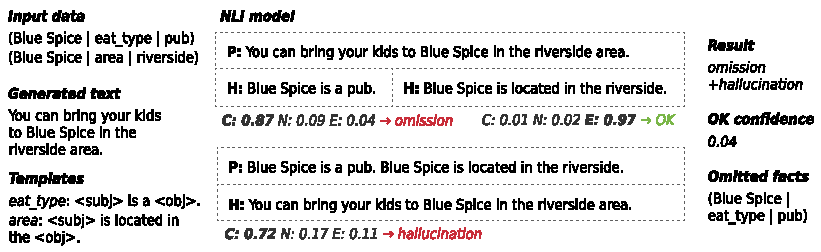
\includegraphics[width=\textwidth]{img/2020_nli_inlg}
    \caption{An example of evaluating the output from a \ac{d2t} system with our metric. The generated text is used as a \textit{premise} (\textit{P}) to check for omissions and as a \textit{hypothesis} (\textit{H}) to check for hallucinations. The \ac{nli} model generates probabilities for \textit{contradiction} (\textit{C}), \textit{neutral} (\textit{N}) and \textit{entailment} (\textit{E}).}
    \label{fig:sem-acc:ex}
\end{figure*}

\paragraph{Checking Semantic Accuracy with NLI} We can use an \ac{nli} model for assessing semantic accuracy of generated texts. Consider the two input facts from \autoref{fig:sem-acc:ex}: $F= $\{\emph{``Blue spice is a pub''}, \emph{``Blue Spice is located in the riverside''}\} and the generated text: $Y= $\emph{``You can bring your kids to Blue Spice in the riverside area.''} We propose using an \ac{nli} model for checking if the semantic information implied by $F$ and $Y$ is equal.
In this case, the model should detect that the first fact is not entailed by the text (there is no mention of Blue Spice being a pub), but the text is also not entailed by the facts (the information about kids is hallucinated).

We achieve this by using the \ac{nli} model to check for entailment in two directions:
\begin{enumerate}
    \item To check for \textrm{omissions}, we use the whole generated text as a premise and sequentially feed each fact as a hypothesis to the \ac{nli} model. Any failed \ac{nli} check is considered an omission.
    \item To check for \textrm{hallucinations}, we concatenate all facts as a premise and feed the generated text as a hypothesis to the \ac{nli} model. If this \ac{nli} check fails, the text is considered to contain hallucination. This step cannot be split into simpler \ac{nli} checks.
\end{enumerate}

The final output of our metric is either 4-way (denoted as \textsc{Fine}) or 2-way (denoted as \textsc{Rough}):
\begin{itemize}
    \item \textsc{Fine}: We output the probabilities of 4 categories: \emph{OK} (i.e., all \ac{nli} checks passed), \emph{omission}, \emph{hallucination}, or \emph{omission+hallucination} (based on the failed checks). The 4-way output is more useful for system evaluation since we can distinguish whether the system tends to hallucinate or omit information.
    \item  \textsc{Rough}: The three failure modes are combined into \emph{not\_OK}. The 2-way output corresponds more to usage inside an \ac{d2t} generation system for output reranking or filtering, where any incorrect should be penalized or filtered out.
\end{itemize}

Additionally, we compute a \textit{confidence score} of the model as the minimum of all the entailment probabilities.


\subsection{Experiments}
\label{sec:sem-acc:experiments}
For our \ac{nli} model, we use the \texttt{roberta-large-mnli}\footnote{\scalebox{0.95}[1.0]{\url{https://huggingface.co/roberta-large-mnli}}} checkpoint of the pretrained RoBERTa model \cite{liuRoBERTaRobustlyOptimized2019}, which was finetuned on the Multi\ac{nli} dataset \cite{williams2018mnli}. We use the model \textit{as is}, without any further training on domain-specific data.
Given a premise text and a hypothesis text, the \ac{nli} model produces a probability distribution over three results: \textit{contradiction}, \textit{neutral},
and \textit{entailment} (see \autoref{sec:sem-acc:method}). We consider a \ac{nli} check as passed if the probability for \textit{entailment} is the highest of the three.


We experiment with the WebNLG and E2E datasets (see \autoref{sec:datasets} for the descriptions of the datasets). Since both datasets were used in shared tasks, we can compare the outputs of our system with the respective measures of semantic accuracy:
\begin{itemize}
    \item For WebNLG, we compare our metric with crowdsourced human ratings of semantic adequacy \cite{shimorinaWebNLGChallengeHuman2019}. In particular, we use the question: \textit{``Does the text correctly represent the meaning in the data?''}, where the human annotators used a three-point Likert scale (1 = Incorrect, 2 = Medium, 3 = Correct). The answers are averaged over multiple annotators. In our experiments, we consider a sentence correct if it achieved a human rating 2.5 or higher.\footnote{We also tried a threshold of 2.0, with slightly worse results.}
    \item For E2E, we compare our metric to the results of the handcrafted automatic script which was used in the E2E challenge \cite{dusekEvaluatingStateoftheartEndtoEnd2020}.\footnote{While the E2E challenge did include crowdsourced evaluation of semantic accuracy, the results were unreliable, overestimating the number of errors \cite{dusekEvaluatingStateoftheartEndtoEnd2020}.} We further use small sets of system outputs and human-written texts with expert annotation \citep[provided by][]{dusekSemanticNoiseMatters2019} to evaluate our approach against gold-standard annotation and to compare to existing semantic accuracy classifiers for E2E data.
\end{itemize}


We evaluate the \emph{Default} and \emph{Backoff} approaches to acquiring templates as described in \autoref{sec:sem-acc:method}. For WebNLG, we obtained templates by delexicalizing human references for single-triple examples from WebNLG training data.\footnote{For each predicate, we choose randomly if more templates are found and use the backoff if no templates are found.} For E2E, we handcrafted eight templates for each predicate in the dataset.

\subsection{Evaluation}
\label{sec:sem-acc:evaluation}

\begin{table}[t]
    \centering \small
    \begin{tabular}{l ccccc>{\hspace{3mm}}ccccc} \toprule
                & \multicolumn{5}{c}{\bfseries WebNLG} & \multicolumn{5}{c}{\bfseries E2E}                                                                                                                  \\
                & \textbf{A}                           & \textbf{R}                        & \textbf{P} & \textbf{F1} & $\mathbf{\rho}$ & \textbf{Af} & \textbf{Ar} & \textbf{R} & \textbf{P} & \textbf{F1} \\\midrule
        Default & 0.775                                & 0.772                             & 0.796      & 0.784       & 0.628           & 0.911       & 0.933       & 0.895      & 0.910      & 0.903       \\
        Backoff & 0.768                                & 0.760                             & 0.793      & 0.776       & 0.637           & 0.846       & 0.874       & 0.913      & 0.768      & 0.834       \\ \bottomrule
    \end{tabular}
    \caption{WebNLG and E2E results, compared to crowdsourced human ratings and the automatic evaluation script, respectively (A = accuracy, Af = \textsc{Fine} accuracy, Ar = \textsc{Rough} accuracy, R = recall, P = precision, F1 = F-measure, $\rho$ = Spearman correlation of confidence scores with human scores).}
    \label{tab:sem-acc:res}
\end{table}



We evaluate our metric in terms of accuracy, precision, recall, and F1-measure (where \emph{not\_OK} samples are treated as positive since we focus on detecting errors). The overall scores for both datasets are summarized in \autoref{tab:sem-acc:res}.
We additionally perform a manual error analysis on a random sample of 100 error examples for each dataset, i.e., examples where our metric gave a different assessment from the ground truth.


% The results for the E2E dataset are better, probably due to the lower lexical variability of the dataset.
% \OD{a možná kvůli tomu, že human eval pro webnlg je trochu zašuměný, ale nevim, jestli se to sem hodí}


% recall is probably more important than precision (not that there are differences)

\paragraph{WebNLG Analysis} The Spearman correlation of our model's confidence scores with the average human scores on the WebNLG dataset is moderate (around 63\%; $p<$1e-10). Our manual error analysis indicates several potential sources of discrepancies:
\begin{enumerate}
    \item The human annotation is somewhat noisy---many correctly rendered outputs do not reach the 2.5 threshold, while some incorrect ones do.
    \item The human annotators also tend to give lower scores to accurate but ungrammatical or poorly organized texts, while our metric tends to rate these texts as \emph{OK}.
    \item Imprecise templates can confuse the \ac{nli} (e.g., for the predicate \emph{nationality}, our extracted template is \emph{\textless{}subj\textgreater{} was \textless{}obj\textgreater{}}, which works well with values such as \emph{French}, but not with \emph{United States}). This is a weak point of our metric, as illustrated by the very small performance difference between the \emph{Default} and \emph{Backoff} setups. However, the issue can be mitigated by a better selection of the templates from training data, e.g., using language-model scoring.
\end{enumerate}

Moreover, our re-examination shows that almost half of the error examples (42 out of 100) were in fact correctly classified by our metric (i.e., their crowdsourced human annotation was incorrect),  so the true performance is most likely higher than the reported numbers.

%  This is similar to $n$-gram-based metrics on this data (\citealp{shimorinaWebNLGChallengeHuman2019} reports 0.59 for BLEU and 0.73 for METEOR), but unlike these metrics, our approach does not require human-written reference texts.

% To further check whether the size of the input affects performance, we computed Spearman correlation of the number of input triples with metric errors. The resulting very low value of -0.05 ($p=$\,0.02, \emph{Default} setting) shows that the metric holds its performance even for more complex WebNLG examples.
%
% On the other hand, heck for different information 


%Third, we note that many examples are dubious, e.g. there are typos in the text or the text interprets the data too loosely. In these cases, the notion of semantic accuracy can differ between the annotators.





\paragraph{E2E Analysis} The results for the E2E dataset are very good compared to the WebNLG dataset, with over 90\% agreement with the handcrafted script. This can be attributed to lower lexical variability and less noisy texts, as well as to the better quality of the handcrafted templates (the difference between the \emph{Default} and \emph{Backoff} setups is much more pronounced here). The main issues identified by our error analysis are:
\begin{enumerate}
    \item Problems in the interpretation of some values, e.g., \textit{price range=less than \textsterling{}20} is verbalized as ``cheap'' or \textit{family-friendly=no} as ``adult-only''. These cases are classified as \emph{not\_OK} by the \ac{nli} model.
    \item Missing or over-greedy patterns in the slot error script, causing annotation errors.
    \item Edge cases: some expressions cannot be interpreted in a straightforward way, e.g., ``high restaurant'' for \emph{pricerange=high} is deemed OK by the \ac{nli} but not by the slot error script.
    \item Expressions in the outputs that do not correspond to input facts, such as ``with full service'', are considered hallucinations by the \ac{nli} but ignored by the slot error script.
\end{enumerate}
Again, we consider about half of the error examples (45 out of 100) as correctly classified by our metric, and thus our metric's performance is probably higher than the reported values.

\subsection{Discussion}

\paragraph{Are there any alternatives to our metric?} The main alternatives to our metric are mostly reference-based, which makes their use-cases different to ours \cite{zhaoMoverScoreTextGeneration2019,sellam2020bleurt,yuanBARTScoreEvaluatingGenerated2021}. Except for PARENT \cite{dhingraHandlingDivergentReference2019} and RoMe \cite{ronyRoMeRobustMetric2022}, these metrics are also not particularly targetting \ac{d2t} generation. Our metric thus remains a major alternative for evaluating semantic accuracy triple-to-text generation. In the future, it can be potentially accompanied by evaluation metrics based on large language models \cite{zhaoInvestigatingTabletoTextGeneration2023,sottanaEvaluationMetricsEra2023,kocmiLargeLanguageModels2023}.

\paragraph{How to improve the metric?} Perhaps surprisingly, the bottleneck of the metric not in the \ac{nli} model, as out-of-the-box \ac{nli} models are generally better and more robust metrics than a specially trained approaches \cite{chenMENLIRobustEvaluation2022}. What can be a bottleneck is determining how to present the structured data to a \ac{plm} -- that is, replacing manual template generation with a more automated approach. In this respect, see the discussion on replacing template generation with \acp{plm} and \acp{llm} in \autoref{sec:pipeline:discussion}.


\section{Token-Level Error Classification}
\label{sec:tok-eval}

\begin{refbox}
    This section is based on the paper \emph{Text-in-Context: Token-Level Error Detection for Table-to-Text Generation} \cite{kasnerTextinContextTokenLevelError2021}, joint work with Simon Mille and Ondřej Dušek, published in the Proceedings of the 14th International Conference on Natural Language Generation (INLG 2021). The work describes our submission to the Shared Task on Evaluating Accuracy in Generated Texts. The project was led by the author of the thesis; Simon Mille provided the rule-based generator and wrote its description.
\end{refbox}


In this section, we present an automatic metric for \ac{d2t} generation that can detect semantic accuracy errors in the generated text on the \emph{token level}. Our metric combines a rule-based \ac{d2t} generation system and \acp{plm}. We first use a rule-based \ac{d2t} generation system to generate all the facts that can be derived from the input. For each sentence we evaluate, we select a subset of relevant facts by measuring their semantic similarity with the examined sentence. For annotating erroneous tokens, we finetune a pretrained language model for token-level classification, using the annotated data with the relevant facts in the context as the ground truth.

On the test set of the Shared Task on Evaluating Accuracy in Generated Texts \cite{thomsonGenerationChallengesResults2021}, we achieve 69\% recall and 75\% precision with a model trained on a mixture of human-annotated and synthetic data, placing first out of four submissions in the track for automatic metrics. The code for our experiments is available on Github.\footnote{\url{https://github.com/kasnerz/accuracySharedTask_CUNI-UPF}}


\subsection{Motivation}
\label{sec:tok-acc:motivation}


In \autoref{sec:sem-acc}, we presented a metric for detecting semantic errors for \ac{d2t} generation at the level of individual data items. The metric is well-suited for cases where the text should mention \emph{all the data on the input}, as it can report individual missing items (omissions). However, it is less suitable for detecting incorrect information in the text (hallucinations), as it can give only a single ``hallucination score'' for the entire text. This is problematic for the texts generated from complex data, where the omissions are not relevant (since we do not verbalize all the input data), but the system can still produce numerous hallucinations.


An example of a dataset with complex data is Rotowire (\citealp{wiseman2017challenges}; see \autoref{sec:datasets} for details). In this dataset, the task is to generate basketball match summaries from tabular data. Rotowire poses multiple challenges for neural systems, including the fact that it requires content selection or that its human-written training texts are themselves not always grounded in data, which makes neural models more susceptible to hallucination.
The output texts are also usually longer, which makes the hallucinations more common and detecting hallucination errors on a more fine-grained level essential.

There is, however, no established way to check for hallucinations automatically. Specific content-checking metrics mostly remain a domain of handcrafted pattern matching \cite{wen2015semantically,dusekSemanticNoiseMatters2019}, which does not scale well to new domains. While human evaluation provides a more reliable alternative, it is costly and difficult to set up \cite{van2019best,belzDisentanglingPropertiesHuman2020,thomsonGoldStandardMethodology2020}. Regarding neural metrics such as BERTScore \cite{zhang2019bertscore} or BLEURT \cite{sellam2020bleurt}, most of them have not been evaluated for content preservation, especially on the level of individual tokens.


\subsection{Shared Task in Evaluating Accuracy}
\label{sec:tok-acc:st}
The goal of the Shared Task on Evaluating Accuracy in Generated Texts at INLG 2021 was to develop a token-level error annotation metric for complex \ac{d2t} generation \cite{reiterSharedTaskEvaluating2020}. The organizers of the shared task first manually annotated 60 outputs of various neural systems trained on Rotowire, using the error types defined in \citet{thomsonGoldStandardMethodology2020}:
\begin{itemize}
    \item \errnum{NUMBER} --  Incorrect number (both digits and numerals).
    \item \errent{NAME} -- Incorrect named entity (people, places, teams, days of the week).
    \item \errword{WORD} -- Incorrect word which is not one of the above.
    \item \errctx{CONTEXT} --  A phrase inappropriate for the context.
    \item \errnc{NOT\_CHECKABLE} --  A statement which cannot be checked.
    \item \errother{OTHER} --  Any other type of mistake.
\end{itemize}
\begin{figure}[t]
    \footnotesize
    \lineacross{}


    The Memphis Grizzlies (5-\errnum{2}) defeated the Phoenix Suns (3 - 2) \errent{Monday} 102-91 at the \errent{Talking Stick Resort Arena} in Phoenix. The Grizzlies had a \errword{strong} first half where they \errword{out-scored} the Suns \errnum{59}-\errnum{42}. Marc Gasol scored 18 points, \errword{leading} the Grizzlies.  \errctx{Isaiah Thomas added} 15 points, he is \errnc{averaging 19 points on the season so far}.
    \vspace{1mm}

    \begin{itemize}
        \item \errnum{2}                                       -- Incorrect number, should be 0.
        \item \errent{Monday}                                  -- Incorrect named entity, should be Wednesday.
        \item \errent{Talking Stick Resort Arena}              -- Incorrect named entity, should be US Airways Center.
        \item \errword{strong}                                 -- Incorrect word, the Grizzlies did not do well in the first half.
        \item \errword{out-scored}                             -- Incorrect word, the Suns had a higher score in first half.
        \item \errnum{59}                                      -- Incorrect number, should be 46.
        \item \errnum{42}                                      -- Incorrect number, should be 52 .
        \item \errword{leading}                                -- Incorrect word.  Marc Gasol did not lead the Grizzlies, Mike Conley did with 24 points.
        \item \errctx{Isaiah Thomas added}                     -- Context error.  Thomas played for the Suns, but context here implies he played for the Grizzlies and added to their score.
        \item \errnc{averaging 10 points on the season so far} -- Not checkable.  This is very hard to check, since data sources report performance per season and per game, not performance up to a particular point in a season.
    \end{itemize}
    \lineacross{}

    \caption{Example text with error annotations adapted from \citet{thomsonGenerationChallengesResults2021}, using the error marking style from \citet{thomsonEvaluatingFactualAccuracy2023}. The original data for this game is available at \url{https://www.basketball-reference.com/boxscores/201411050PHO.html} .}
    \label{fig:tok-eval:example}
\end{figure}
An example of an annotated system output is provided in \autoref{fig:tok-eval:example}. The objective of the shared task was to either implement an automatic metric for creating the same type of annotations automatically or to develop a human evaluation scenario capable of producing the same annotations while requiring fewer resources.


% Our submission for the shared task falls into the first category:
% we developed an automatic metric for token-level error annotation which combines a rule-based generation system with a neural retrieval model and a pretrained neural LM used for error tagging.
% We evaluated our approach in a cross-validation scenario to select the best configuration for the shared task. Overall, our system is able to reach 65\% error detection F1 score and ranked first out of four automatic submissions in the shared task.



\subsection{Our System}
\label{sec:tok-eval:system}

\begin{figure*}[ht]
    \centering
    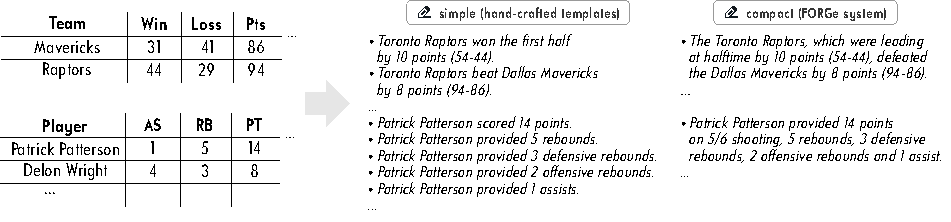
\includegraphics[width=\textwidth]{img/tok-eval_generator.pdf}
    \caption{Rule-based NLG which we use to generate facts from the input data. The facts are used as an input to the error checking model (see Figure \ref{fig:tok-eval:system}). We experiment with (a) simple hand-crafted templates and (b) compact sentences generated by the FORGe system.}
    \label{fig:tok-eval:gen}
\end{figure*}





Our submission for the shared task falls into the first category: we developed an automatic metric based on a \ac{plm}, which marks each token in the output text for the presence of errors. To make the tabular data understandable for the \ac{plm}, we use a rule-based system to exhaustively generate all the facts that can be derived from the data. Since the context window of the \ac{lm} is limited, we also use a neural-based retrieval system to retrieve only $c$ relevant facts, which are added into the context window of the \ac{lm} to support its decisions. We describe individual components of our system below.

% We developed an automatic metric for token-level error annotation which combines (1) a rule-based sentence generation system, (2) a neural retrieval model, and (3) a pretrained encoder \ac{lm} used for error tagging. The idea behind our system is that the pretrained encoder will compare the output with the relevant context retrieved from the data, tagging errors on the token level.

% Our system is composed of three steps, which we describe below:
% \begin{enumerate}
% \item A rule-based generator for fact descriptions,
% \item A retrieval system for selecting facts relevant for a given sentence,
% \item A token-level error tagger.
% \end{enumerate}


\paragraph{Rule-based Fact Descriptions}
We use a rule-based system to generate facts from the input tables in natural language. For each game, we generate facts about the game (hosting team, visiting team, date converted to weekday), line-score objects (team name and statistics), and box-score objects (player name, player team, player starting position and their personal statistics). We also generate additional facts that can be inferred from the input table, such as which team won and by how much, comparisons between the team and player raw data (e.g., \emph{Team A and Team B committed the same number of fouls}), details based on statistics (e.g., \emph{Player X recorded a double-double}), or an interpretation of some numbers (e.g., \emph{Team A came back in the 4th quarter}).\footnote{A number of facts frequently mentioned in human-written descriptions could not be obtained from the Rotowire data, as for instance the player stats per quarter, a career-high points total, whether a player is an all-star or not, or if a player scored the winning shot.}

We experiment with both \emph{simple} descriptions created by filling in sentence templates and \emph{compact} descriptions generated using a grammar-based system:
\begin{itemize}
    \item \textbf{Simple descriptions} are produced by a template-based system, with one template per fact. We handcrafted 129 sentence templates to cover all the facts described above. A sentence template looks like the following: ``\textit{[PLAYER$\_$NAME] scored [PTS] points.}'', where square brackets indicate variables that are instantiated with the corresponding input values (see Figure~\ref{fig:tok-eval:gen} for sample sentences).
    \item  \textbf{Compact descriptions} are produced by the FORGe system \cite{mille2019teaching}, which allows for the generation of more compact sentences.  For instance, the five bottom sentences from the simple system in \autoref{fig:tok-eval:gen} are covered by the single bottom sentence from the compact system. FORGe performs surface realization in several steps, by first aggregating the templates based on the predicate and argument identity and then structuring, linearizing, and inflecting components of the sentences. The FORGe grammars were used off-the-shelf,\footnote{We deactivated cross-sentence referring expression generation so that each generated sentence can be used independently.} with additional 98 manually crafted abstract templates.
\end{itemize}

The simple system produces about 569 facts for each game. The compact system covers the same amount of information with more syntactically complex sentences, producing about 112 sentences per game, i.e., five times less.


\begin{figure*}[t]
    \centering
    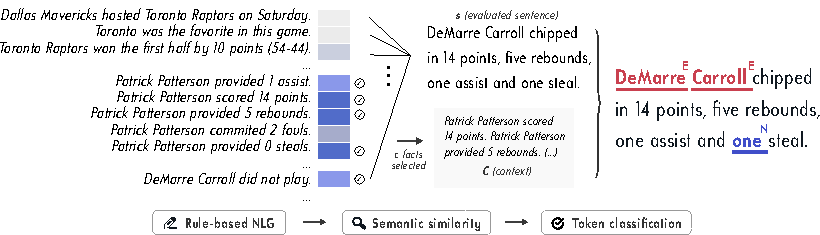
\includegraphics[width=\textwidth]{img/tok-eval_system.pdf}
    \caption{An overview of our system. First, we generate the facts from the input table with a rule-based NLG system (see Figure \ref{fig:tok-eval:system}). For each evaluated sentence $s$, we select $c$ facts with the highest semantic similarity, getting a context $C$. The pair $(C, s)$ is given as an input to a pretrained LM for token-level error classification.}
    \label{fig:tok-eval:system}
\end{figure*}

\paragraph{Context Retrieval} The maximum length of the input sequence for our error tagger is 512 tokens, which is about 10\% of the total length of the generated sentences $G$. Therefore, we select only a subset of $G$, which we refer to as \emph{context} $C$. For each generated sentence $g_i\in G$, we measure semantic similarity between $g_i$ and the evaluated sentence $s$ using Sentence Transformers \cite{reimers-gurevych-2019-sentence}. In particular, we embed the sentence tokens by applying mean pooling on the output of \texttt{paraphrase-distilroberta-base-v2}, getting the embedding vectors $e_{s}$ and $e_{g_i}$. Then, we compute the cosine similarity between the embeddings:
\begin{align}
    score = \frac{e_s \cdot e_{g_i}}{\lVert e_s \rVert \lVert e_{g_i} \rVert}.
\end{align}
For the context $C$, we select the top $c$ sentences from $G$ that have the highest cosine similarity to $s$.


\paragraph{LM-based Error Tagger}
As our error tagger, we use RoBERTa \cite{liuRoBERTaRobustlyOptimized2019} with a token-level classification head. The model receives an input $X = (C, s)$ and is trained to annotate each token in $s$ either with an \textit{OK} label or with a label corresponding to one of the error categories. We experiment with two data sources for training the model:
\begin{itemize}
    \item \emph{gold-standard annotated data} from the shared task (which contains all error types),
    \item \emph{synthetic data} created by perturbing the human-written summaries from Rotowire (which contains only \errent{NAME} and \errnum{NUMBER} errors).
\end{itemize}
% For our submission, we use two-stage finetuning: first we finetune on synthetic data, then we finetune on the annotated data. 
% \ODdel{A cross-validation on the development set gives us 65\% F1-score (61\% precision and 69\% recall).}\OD{I'd include at least bits of the mega-table instead.}

\paragraph{Synthetic Data} The gold-standard data contains only 60 games, as opposed to 3,395 games in the Rotowire training set. This led us to the idea of using the training set as a source of synthetic data, introducing errors into human-written descriptions. We focus only on the \errent{NAME} and \errnum{NUMBER} errors, i.e., the categories that are the most represented and also easiest to generate. In each sentence, we identify named entities in the text using \emph{spaCy}.\footnote{\url{https://spacy.io}} We modify only a certain portion of entities according to the \emph{entity modification rate} (EMR), which we treat as a hyperparameter. We introduce the \errent{NAME} errors by:
\begin{enumerate}
    \item swapping the names of teams with opponent teams,
    \item swapping the names of players with other players in the game,
    \item swapping the names of cities with other cities in the Rotowire dataset,
    \item modifying the days of the week.
\end{enumerate}
For \errnum{NUMBER} errors, we take an integer $n$ identified in the text, sample a number from a normal distribution with $\mu=n$ and $\sigma=3$, and truncate it to get an integer. We re-sample if the output equals the original number or for negative outputs. If the number is spelled out, we use \texttt{text2num}\footnote{\url{https://pypi.org/project/text2num/}} and  \texttt{num2words}\footnote{\url{https://pypi.org/project/num2words/}} to convert to digits and back.


\subsection{Experiments}
\label{sec:tok-eval:experiments}

We train a PyTorch version of RoBERTa from the Huggingface Transfomers repository \cite{wolf2019HuggingFacesTS} using the AdamW optimizer \cite{loshchilov2018fixing}, learning rate $5\times10^{-5}$ and linear warmup.
% $\beta_1=0.9, \beta_2=0.997, \epsilon=10^{-8}$, 
We finetune the model for 10 epochs and select the model with the highest validation score.
We experiment with several hyperparameters: % regarding our training data: 
\begin{itemize}
    \item \emph{simple} vs.~\emph{compact} sentences in $G$, % (Section \ref{sec:rule-based-system})
    \item  \textit{number of sentences} retrieved for the context: $c$ = 5, 10, 20 or 40;
    \item \textit{entity modification rate} (EMR): proportion of entities modified in the synthetic data: 0.25, 0.5, or 0.75.
\end{itemize}
We evaluate the model using a script provided by the organizers, which computes recall and precision of the model output with respect to the human-annotated data. Since we use the human-annotated data for training, we perform 6-fold cross-validation: in each run, we use 45 games for training, 5 games for validation, and 10 games for evaluation.


\begin{table*}[!htbp]
    \centering\footnotesize
    \begin{tabular}{@{}l l r >{\hspace{2mm}} ccc >{\hspace{2mm}} ccc >{\hspace{2mm}} ccc@{}}\toprule
        \multirow{2}{*}{\bf Gen.}                    & \multirow{2}{*}{\bf Data} & \multirow{2}{*}{$c$} & \multicolumn{3}{c}{\bf EMR = 0.25} & \multicolumn{3}{c}{\bf EMR = 0.5} & \multicolumn{3}{c}{\bf EMR = 0.75}                                                         \\
                                                     &                           &                      & R                                  & P                                 & F1                                 & R         & P     & F1    & R         & P     & F1    \\\midrule
        \multirow{8}{*}{\bf\rotatebox{90}{Simple} }  & \multirow{4}{*}{s}
                                                     & 5                         & 0.123                & 0.723                              & 0.210                             & 0.165                              & 0.512     & 0.250 & 0.310 & 0.323     & 0.316         \\
                                                     &                           & 10                   & 0.138                              & 0.737                             & 0.232                              & 0.181     & 0.549 & 0.272 & 0.328     & 0.400 & 0.360 \\
                                                     &                           & 20                   & 0.137                              & \bf 0.741                         & 0.231                              & 0.179     & 0.559 & 0.271 & 0.327     & 0.433 & 0.373 \\
                                                     &                           & 40                   & 0.165                              & 0.712                             & 0.268                              & 0.199     & 0.560 & 0.294 & 0.296     & 0.436 & 0.353 \\\cdashlinelr{2-12}
                                                     & \multirow{4}{*}{s+h}
                                                     & 5                         & 0.422                & 0.617                              & 0.501                             & 0.414                              & 0.594     & 0.488 & 0.401 & 0.583     & 0.475         \\
                                                     &                           & 10                   & 0.467                              & 0.551                             & 0.506                              & 0.438     & 0.638 & 0.519 & 0.428     & 0.665 & 0.521 \\
                                                     &                           & 20                   & 0.518                              & 0.640                             & 0.573                              & 0.544     & 0.575 & 0.559 & 0.509     & 0.595 & 0.549 \\
                                                     &                           & 40                   & 0.584                              & 0.644                             & \bf 0.613                          & \bf 0.595 & 0.612 & 0.603 & 0.519     & 0.639 & 0.573 \\\midrule
        \multirow{8}{*}{\bf \rotatebox{90}{Compact}} & \multirow{4}{*}{s}
                                                     & 5                         & 0.151                & \bf 0.696                          & 0.248                             & 0.170                              & 0.617     & 0.267 & 0.336 & 0.427     & 0.376         \\
                                                     &                           & 10                   & 0.176                              & 0.663                             & 0.278                              & 0.195     & 0.624 & 0.297 & 0.295     & 0.486 & 0.367 \\
                                                     &                           & 20                   & 0.196                              & 0.672                             & 0.303                              & 0.205     & 0.635 & 0.310 & 0.278     & 0.552 & 0.370 \\
                                                     &                           & 40                   & 0.166                              & 0.643                             & 0.264                              & 0.197     & 0.595 & 0.296 & 0.306     & 0.530 & 0.388 \\ \cdashlinelr{2-12}
                                                     & \multirow{4}{*}{s+h}
                                                     & 5                         & 0.600                & 0.641                              & 0.620                             & 0.552                              & 0.635     & 0.591 & 0.588 & 0.600     & 0.594         \\
                                                     &                           & 10                   & 0.583                              & 0.662                             & 0.620                              & 0.629     & 0.606 & 0.617 & \bf 0.656 & 0.606 & 0.630 \\
                                                     &                           & 20                   & 0.622                              & 0.647                             & 0.634                              & 0.597     & 0.688 & 0.639 & 0.600     & 0.660 & 0.629 \\
                                                     &                           & 40                   & 0.614                              & 0.690                             & \bf \phantom{*}0.650*              & 0.609     & 0.630 & 0.619 & 0.611     & 0.630 & 0.620 \\\bottomrule
    \end{tabular}
    \caption{Recall (R), precision (P) and F1 scores on development data. $s$ stands for synthetic training data and $h$ for human training data.  $c$ indicates the number of sentences in the context provided to the tagger, EMR stands for entity modification rate. Best recall, precision and F1 scores for both generators (simple and compact) are shown in bold, the submitted model is identified by an asterisk (*).}
    \label{tab:tok-eval:results}
\end{table*}

\paragraph{Development Results} The results of our model on the development data are listed in Table \ref{tab:tok-eval:results}.\footnote{Due to space constraints, we do not list the results of model trained only on annotated data. The results were overall in the 0.3-0.5 range for both recall and precision, and no model was the best-performing one in terms of any metric.} For our final submission, we selected the model with the best F1-score overall, which is 0.65 (61\% recall and 69\% precision). The model uses 40 compact sentences in context, 0.25 EMR, and was trained on both synthetic and human-annotated data. Although compact texts are generally helpful, there are also some well-performing models using simple templates only. A higher number of sentences in context may help to achieve better F1-score, but not always (the longer context is also sometimes cropped to fit the input). Using a higher EMR then generally leads to higher recall, suggesting that the model adapts to the base rate of errors.

\begin{table}[t]
    \centering\small
    \begin{tabular}{l cccc}\toprule
        \multirow{2}{*}{\bf Error Type} & \multicolumn{2}{c}{\bf Mistake} & \multicolumn{2}{c}{\bf Token}                 \\
                                        & R                               & P                             & R     & P     \\ \midrule
        \errent{NAME}                   & 0.750                           & 0.846                         & 0.759 & 0.862 \\
        \errnum{NUMBER}                 & 0.777                           & 0.750                         & 0.759 & 0.752 \\
        \errword{WORD}                  & 0.514                           & 0.483                         & 0.465 & 0.529 \\
        \errctx{CONTEXT}                & 0.000                           & -                             & 0.000 & -     \\
        \errnc{NOT\_CHECKABLE}          & 0.000                           & -                             & 0.000 & -     \\
        \errother{OTHER}                & 0.000                           & -                             & 0.000 & -     \\ \noalign{\vskip 0.1cm}\hdashline\noalign{\vskip 0.1cm}
        \textbf{Overall}                & 0.691                           & 0.756                         & 0.550 & 0.769 \\\bottomrule
    \end{tabular}
    \caption{Results of our system on test data: recall (R) and precision (P) are shown for individual error types.}
    \label{tab:tok-eval:results-test}
\end{table}

\paragraph{Submission Results}
Table \ref{tab:tok-eval:results-test} shows the results of our model on the official test data of the task, broken down by error types. The overall scores are higher than on the development set -- test set recall is 0.691 (vs.~0.614 on the development set), and precision is 0.756 (vs.~0.690). The fact that we used all the available human-annotated data for training the final model may have contributed to the difference, but it is also possible that the test data was somewhat less challenging. We note that our model was able to identify only three types of errors (\errent{NAME}, \errnum{NUMBER}, \errword{WORD}), having better results for the \errent{NAME} and \errnum{NUMBER} errors. We believe the explanation is two-fold: the names and numbers are often found verbatim in the input data (and in our generated facts), which makes them easy to detect, and also the corresponding error types were the most represented in the training data. In contrast, the three error types that were not detected are much less represented in the training data and hard to detect in our setup.


\subsection{Discussion}
\paragraph{What are the limitations of our metric?} Firstly, our metric depends on the existence of a rule-based system for generating factual statements from the data. Such a system may be hard to develop, even though we have shown that simple templates can be similarly efficient as more complex approaches. As our approach is data-driven, it also requires the system outputs annotated with errors. This requirement may be partially mitigated by using synthetic data. In our case, using synthetic data only results in low recall (see \autoref{tab:tok-eval:results}), but we believe that more sophisticated techniques for creating the synthetic data could help to achieve better results.

\paragraph{How to improve our metric?} Our submission achieved the best results in the automatic metrics category, but there is still a gap with what humans can achieve, as shown by the Laval University submission's overall 0.841 recall and 0.879 precision \cite{garneau2021laval}. One way to improve our system would be to enrich the reference fact descriptions, by either inferring more information from the raw data, or by extracting additional data from external databases. Another option would be to add surrounding sentences to the context -- this could help to resolve coreferences (e.g., if a player is referred to as \textit{"He"}) and to detect the \errctx{CONTEXT} errors.

\paragraph{Are there any alternatives?} Recently, the evaluation metrics based on \acp{llm} are starting to provide an alternative, more flexible approach for evaluting generated texts \cite{zhaoInvestigatingTabletoTextGeneration2023,sottanaEvaluationMetricsEra2023,chiang-lee-2023-large,fu2023gptscore}. An advantage of the \ac{llm}-based metrics is the possibility of defining custom error categories without the need for having annotated data for finetuning the model. We explore such an approach in \autoref{sec:quintd}, where we use a \ac{llm}-based metric for token-level evaluation of generated text. However, it should be noted that with \ac{llm}-based metrics, greater flexibility is traded for lower controllability, especially in the case of closed-source models. Such an evaluation can be thus biased and non-reproducible \cite{stureborgLargeLanguageModels2024,kooBenchmarkingCognitiveBiases2023,wangLargeLanguageModels2023}.

\section{Conclusion}
We introduced two metrics for evaluating semantic accuracy of \ac{d2t} generation. The metric presented in \autoref{sec:sem-acc} targets the cases where all the data items need to be mentioned in the output text. The metric uses a combination of simple templates and an off-the-shelf neural model, make our approach applicable with minimal additional efforts. The metric introduced in \autoref{sec:tok-eval} then targets complex data-to-text generation, enabling annotating factual errors on the level of individual tokens.